% Provenance (never printed): see sources/outline_sources.md (Year 2: the Himalaya and Tibet;
% the Andes; crustal thickening and plateaus). Himalayan units, thrusts and rates after Lave
% and Avouac (2000), Ader et al. (2012), Cattin et al. (2001), Dong et al. (2026, STDS);
% Asian extrusion after Jiao et al. (2023); Tibetan rifts after Wang et al. (2021); Central
% Andes after Gerbault et al. (2005); flat slabs after Gauthier et al. (2024). Relief from
% ETOPO1 (figdata/bachelor-2/plateaus.py); plate velocities from NNR-MORVEL56 (Book 2 ledger
% row nnr56:poles). Exercise and problem values in the Book 4 scratch calculator
% calc/ch14.py.
\chapter{Collision and Andean Belts Compared}\label{ch:b2:himalaya-andes}

Two plateaus on Earth stand more than four kilometres high over hundreds of kilometres.
Tibet was raised where India ran into Asia, two continents meeting after the ocean between
them had gone. The Altiplano was raised where an ocean plate, the Nazca plate, still slides
beneath South America, with no continent arriving at all. Two different engines built two
similar landforms. This chapter takes the two belts apart, measures how thick their crust
has become and why, and asks what stops them from growing higher.
% ledger: lave00:setting, gerbault05:andes, data:b4-etopo-tibet, data:b4-etopo-andes

\begin{recall}
\textbf{From the high-school volume}: continental collision and the suture; India's
northward drift, its slowdown and the debated age of the collision; the Tibetan Plateau about
\qty{4600}{m} high over a crust about \qty{70}{km} thick. \textbf{From the Year 1 volume}:
Airy isostasy and the Bouguer slab; active margins, the subducting slab, the volcanic arc and
the arc--trench gap; plate velocities from angular velocities; Byerlee's law; the moment
magnitude. \textbf{From \cref{ch:b2:crustal-melting}}: Himalayan \omterm{def:b2:crustal-melting:leucogranite}{leucogranites}.
\textbf{From \cref{ch:b2:alpine-orogen}}: \omterm{def:b2:alpine-orogen:orogen}{orogen}, \omterm{def:b2:alpine-orogen:nappes}{nappe}, \omterm{def:b2:alpine-orogen:decollement}{décollement}, thin- and
\omterm{def:b2:alpine-orogen:skin}{thick-skinned tectonics}, \omterm{def:b2:alpine-orogen:ftb}{fold--thrust belt}, \omterm{def:b2:alpine-orogen:foreland}{foreland basin}, \omterm{def:b2:alpine-orogen:balanced}{balanced cross-sections}.
\end{recall}

\begin{definition}[Collision orogen; Andean-type orogen]\label{def:b2:himalaya-andes:types}
A \emph{collision orogen}\index{collision orogen} is an \omterm{def:b2:alpine-orogen:orogen}{orogen} built by the convergence of
two continental margins after the ocean between them has been consumed; its axis is a suture.
An \emph{Andean-type orogen}\index{Andean-type orogen} is an \omterm{def:b2:alpine-orogen:orogen}{orogen} built on the overriding
plate of an ocean--continent subduction zone, while subduction goes on beneath it; its axis
is a volcanic arc.
\end{definition}


\section{India against Asia}\label{sec:b2:himalaya-andes:himalaya}

India met the southern edge of Eurasia about 50 million years ago along the Indus--Tsangpo
suture, also called the Indus--Yarlung suture; the exact date is still debated, as the
high-school volume showed. Convergence did not stop. Today India and Asia approach each other
at about \qty{40}{mm} a year; from the angular velocities of the NNR-MORVEL56 plate model,
India moves at \qty{45}{mm} a year relative to Eurasia at \ang{28}~N, \ang{85}~E, towards
\ang{22} east of north. Only part of that motion is taken up in the Himalaya. Across Nepal,
GPS stations show India and southern Tibet converging at $17.8 \pm \qty{0.5}{mm}$ a year in the
centre and east and $20.5 \pm \qty{1}{mm}$ a year in the west: about half of the total. The rest
is spread over Tibet and the rest of Asia.
% ledger: lave00:setting, najman21:collision-age, jiao23:extrusion, nnr56:poles, ader12:rates, ader12:mht
% values (plateaus.py): v_india_eurasia 44.99 mm/yr, azimuth 21.65

The maps below show the two belts with the same contours, and the swaths along which this
chapter cuts them.

\begin{omfigure}
\centering
% ledger: data:b4-etopo-tibet, data:b4-etopo-andes
\begin{tikzpicture}
\begin{axis}[name=tib, scale only axis, width=8.0cm, height=4.8cm, xmin=75, xmax=100,
  ymin=25, ymax=40, xlabel={longitude (\unit{\degree} E)}, ylabel={latitude (\unit{\degree} N)},
  tick label style={font=\scriptsize}, label style={font=\small}, xtick={75,80,...,100},
  ytick={25,30,...,40}, title={\small Himalaya and Tibet}]
\addplot[omThm!35, line width=0.3pt] table[x=lon, y=lat] {figdata/out/bachelor-2-plateaus-tc2000.dat};
\addplot[omThm!90!black, line width=0.4pt] table[x=lon, y=lat] {figdata/out/bachelor-2-plateaus-tc4000.dat};
\draw[black, densely dashed, line width=0.9pt] (axis cs:86,25) rectangle (axis cs:90,40);
\node[font=\scriptsize, fill=white, fill opacity=0.85, text opacity=1, inner sep=1pt] at (axis cs:80,26.2) {Ganges plain};
\node[font=\scriptsize, fill=white, fill opacity=0.85, text opacity=1, inner sep=1pt] at (axis cs:94.5,33.5) {Tibetan Plateau};
\node[font=\scriptsize, fill=white, fill opacity=0.85, text opacity=1, inner sep=1pt] at (axis cs:83,39.2) {Tarim};
\end{axis}
\begin{axis}[at={(tib.east)}, anchor=west, xshift=1.6cm, scale only axis, width=3.6cm,
  height=4.8cm, xmin=-75, xmax=-60, ymin=-30, ymax=-10,
  xlabel={longitude (\unit{\degree})}, tick label style={font=\scriptsize},
  label style={font=\small}, xtick={-75,-70,-65,-60}, ytick={-30,-25,...,-10},
  title={\small Central Andes}]
\addplot[blue!60!black, line width=0.45pt] table[x=lon, y=lat] {figdata/out/bachelor-2-plateaus-ac0.dat};
\addplot[omThm!35, line width=0.3pt] table[x=lon, y=lat] {figdata/out/bachelor-2-plateaus-ac2000.dat};
\addplot[omThm!90!black, line width=0.4pt] table[x=lon, y=lat] {figdata/out/bachelor-2-plateaus-ac4000.dat};
\draw[black, densely dashed, line width=0.9pt] (axis cs:-75,-21) rectangle (axis cs:-60,-19);
\node[font=\scriptsize, fill=white, fill opacity=0.85, text opacity=1, inner sep=1pt] at (axis cs:-73,-25) {Pacific};
\end{axis}
\end{tikzpicture}
\par\smallskip{\small Relief of the two belts from ETOPO1, every node \qty{0.1}{\degree}
apart: contours at \qty{2000}{m} (light) and \qty{4000}{m} (dark), and the coastline on the
right. Latitudes on the right are negative south of the equator, longitudes negative west of
Greenwich. The dashed boxes are the swaths of the profiles further on: \qtyrange{86}{90}{\degree} E
across the Himalaya and Tibet, \qtyrange{19}{21}{\degree} S across the Central Andes.}
\end{omfigure}

\subsection{The units and the thrusts}

From the Ganges plain northwards, a traverse of the Himalaya crosses a pile of thrust sheets
cut from India's northern margin, separated by faults that run the length of the range.
\begin{itemize}
\item The \emph{Indo-Gangetic foredeep} is the Himalayan \omterm{def:b2:alpine-orogen:foreland}{foreland basin}; it traps part of
the debris eroded from the range.
\item The \emph{sub-Himalaya}, the Siwalik Hills, is made of the \omterm{def:b2:alpine-orogen:foreland}{molasse} of that basin,
claystones to conglomerates of late Miocene to Pleistocene age, 3500 to \qty{5500}{m} thick,
laid down between 14 and \qty{1}{Ma}, then scraped off at the range front and folded above a
\omterm{def:b2:alpine-orogen:decollement}{décollement}: a thin-skinned \omterm{def:b2:alpine-orogen:ftb}{fold--thrust belt}. Its southern edge is the \emph{Main Frontal
Thrust} (MFT).
\item The \emph{Lesser Himalaya}, rocks of medium metamorphic grade, lies between the
\emph{Main Boundary Thrust} (MBT) below and the \emph{Main Central Thrust} (MCT) above.
\item The \emph{Greater Himalayan sequence} (the High Himalaya) above the MCT is made of
high-grade metamorphic rocks, partly molten: the \omterm{def:b2:crustal-melting:migmatite}{migmatites} and \omterm{def:b2:crustal-melting:leucogranite}{leucogranites} of
\cref{ch:b2:crustal-melting}, melted about 30 million years after the collision.
\item The \emph{Tethyan Himalayan sequence}, unmetamorphosed or weakly metamorphosed
sediments of India's old passive margin, rests on the Greater Himalayan sequence along the
\emph{South Tibetan Detachment System} (STDS), the only normal fault among the great
east--west fault zones of the range, more than \qty{2000}{km} long.
\item North of them comes the suture, and beyond it the Asian crust of southern Tibet.
\end{itemize}
% ledger: lave00:setting, lave00:siwaliks, weinberg16:himalaya, dong26:stds

The faults young southwards. The deformation front moved south as one thrust after another
took over, from the Kangmar thrust to the MCT, then the MBT, and now the MFT, which in
central Nepal is the only active structure of the sub-Himalaya. It is the same outward
migration as in the Alps of \cref{ch:b2:alpine-orogen}, written here in rocks that are still
moving. The STDS adds a surprise: a normal fault, extension, inside a range that is being
shortened. It shows that compression and extension can work at the same time in one \omterm{def:b2:alpine-orogen:orogen}{orogen},
at different levels, and it helped bring the hot rocks of the Greater Himalayan sequence up
from the root of the range.
% ledger: lave00:setting, lave00:mft-rate, dong26:stds

\subsection{One fault beneath the range}

The thrusts at the surface root into a single gently dipping fault, the \emph{Main
Himalayan Thrust} (MHT), along which the Indian plate is pushed under the range. It reaches
the surface at the MFT, runs as a flat beneath the Lesser Himalaya, steepens into a ramp at
the front of the High Himalaya, and continues north beneath southern Tibet. Over the Holocene
the folding of river terraces across the Siwaliks records $21 \pm \qty{1.5}{mm}$ a year of
shortening on the MFT, the same as the geodetic rate across the whole range. The MHT is
locked from the surface to about \qty{100}{km} down dip, at 15 to \qty{20}{km} depth; further
north it creeps. The locked part stores the convergence as elastic strain and gives it back
in great earthquakes, such as the Assam earthquake of 1950, of moment magnitude about~8.5.
% ledger: ader12:mht, lave00:setting, lave00:mft-rate, ader12:quakes

\begin{omfigure}
\centering
\begin{tikzpicture}[x=0.6cm, y=0.5cm, font=\scriptsize]
% Indian crust below the MHT and the foredeep
\fill[gray!15] (0,-0.4) -- (5,-0.8) -- (12,-1.6) -- (14,-3.2) -- (24,-4.2) -- (24,-8.5) -- (0,-5.5) -- cycle;
% mantle
\fill[gray!35] (0,-5.5) -- (24,-8.5) -- (24,-9.3) -- (0,-6.3) -- cycle;
% foredeep
\fill[yellow!35] (0,0) -- (4,0) -- (5,-0.8) -- (0,-0.4) -- cycle;
% Siwaliks
\fill[orange!35] (4,0) -- (5,0.6) -- (6.5,0.8) -- (7.6,-1.1) -- (5,-0.8) -- cycle;
% Lesser Himalaya
\fill[green!20] (6.5,0.8) -- (8.5,1.3) -- (11,2.0) -- (13,-2.4) -- (12,-1.6) -- (7.6,-1.1) -- cycle;
% Greater Himalayan sequence
\fill[omThm!35] (11,2.0) -- (12.5,3.6) -- (13.5,4.2) -- (15,3.6) -- (19.53,0.2) -- (20.2,-3.82)
  -- (14,-3.2) -- (13,-2.4) -- cycle;
% Tethyan Himalayan sequence
\fill[cyan!20] (15,3.6) -- (17,3.5) -- (19,3.4) -- (19.53,0.2) -- cycle;
% Asian crust
\fill[orange!15] (19,3.4) -- (24,3.4) -- (24,-4.2) -- (20.2,-3.82) -- cycle;
% leucogranites
\fill[pink!70!red!45] (14.2,2.2) ellipse (0.45 and 0.35);
\fill[pink!70!red!45] (16.6,1.0) ellipse (0.4 and 0.3);
% surface
\draw[line width=0.5pt] (0,0) -- (4,0) -- (5,0.6) -- (6.5,0.8) -- (8.5,1.3) -- (11,2.0) -- (12.5,3.6)
  -- (13.5,4.2) -- (15,3.6) -- (17,3.5) -- (19,3.4) -- (24,3.4);
% faults
\draw[thick] (6.5,0.8) -- (7.6,-1.1);
\draw[thick] (11,2.0) -- (13,-2.4);
\draw[thick, densely dashed] (15,3.6) -- (19.53,0.2);
\draw[thick] (19,3.4) -- (20.2,-3.82);
% MHT
\draw[very thick, red!70!black] (4,0) -- (5,-0.8) -- (12,-1.6) -- (14,-3.2) -- (24,-4.2);
\node[red!70!black, anchor=north] at (8.8,-1.25) {MHT, locked flat};
\node[red!70!black, anchor=north east] at (13.2,-2.6) {ramp};
\node[red!70!black, anchor=north] at (19.5,-4.0) {MHT, creeping};
% Moho
\draw[dashed] (0,-5.5) -- (24,-8.5);
\node[anchor=south west] at (0.2,-5.45) {Indian Moho};
\node at (12,-5.6) {Indian crust};
\node at (16,-7.9) {mantle};
% unit labels
\node[anchor=south] at (1.8,0.05) {foredeep};
\node at (5.6,0.05) {Siw.};
\node at (9.3,0.5) {Lesser Himalaya};
\node[align=center] at (15.6,-0.9) {Greater Himalayan\\sequence};
\node[align=center] at (18.1,2.65) {Tethyan\\Himalaya};
\node at (21.8,0.2) {Asian crust};
% fault labels
\node[anchor=south, font=\scriptsize\bfseries] (mft) at (3.2,1.6) {MFT};
\draw[->] (mft.south) -- (3.95,0.1);
\node[anchor=south, font=\scriptsize\bfseries] (mbt) at (5.9,2.3) {MBT};
\draw[->] (mbt.south) -- (6.5,0.95);
\node[anchor=south, font=\scriptsize\bfseries] (mct) at (10.2,3.6) {MCT};
\draw[->] (mct.south) -- (11.0,2.15);
\node[anchor=south, font=\scriptsize\bfseries] (stds) at (16.6,5.0) {STDS};
\draw[->] (stds.south) -- (15.8,3.1);
\node[anchor=south, font=\scriptsize\bfseries] (sut) at (20.6,5.0) {suture};
\draw[->] (sut.south) -- (19.2,2.4);
\draw[-{Latex[length=2mm]}] (1.2,2.4) -- (0.2,2.4);
\node[anchor=south] at (0.7,2.4) {S};
\draw[-{Latex[length=2mm]}] (22.8,5.0) -- (23.8,5.0);
\node[anchor=south] at (23.3,5.0) {N};
\end{tikzpicture}
\par\smallskip{\small A schematic section across the Himalaya of Nepal (not to scale). The
thrusts young southwards from the MCT to the MBT and the MFT, all rooted in the Main
Himalayan Thrust (MHT), locked beneath the Lesser Himalaya and creeping beneath southern
Tibet; the STDS (dashed) is a normal fault. \omterm{def:b2:crustal-melting:leucogranite}{Leucogranites} (pink) in the Greater Himalayan
sequence; Siw., the Siwaliks. The Indian Moho deepens northwards beneath the range.}
\end{omfigure}
% ledger: lave00:setting, ader12:mht, dong26:stds, weinberg16:himalaya, cattin01:crust

How did the Greater Himalayan sequence, partly molten at depth, come to stand between a
thrust below and a normal fault above? One hypothesis, \emph{channel flow}, has the hot,
weak middle crust flowing out southwards between the two shear zones, drawn up towards the
surface where erosion is fastest. It is a hypothesis: the share of channel flow, collapse
and delamination in the building of the Himalaya and Tibet is still contested.
% ledger: gerbault05:delamination, jiao23:extrusion, dong26:stds

The range does not float freely. Gravity profiles across Nepal show the Bouguer anomaly
falling from about $-40$ to \qty{-500}{mGal} from the Ganges plain to Tibet. Far from the
range, local Airy isostasy holds; near it, the foreland is overcompensated and the high
range undercompensated: the Indian plate is bent down like a beam under the load of the
mountains and holds them up in part by its own stiffness, a regional support whose study
belongs to the Year 3 volume.
% ledger: cattin01:crust

\begin{inthefield}[Measuring a mountain belt that moves]
A geodesy team in the Himalaya sets up permanent GPS stations: an antenna bolted to bedrock
or to a concrete pillar, a receiver, a solar panel, a battery. Each station records its
position every day. One day's position scatters by millimetres, and the noise is not purely
random: it wanders over weeks and seasons. The team therefore models the noise, white plus
coloured, before fitting a straight line to years of daily positions; the slope is the
station's secular velocity, with an honest uncertainty. Across Nepal, about thirty stations
watched for some twenty years show velocities that fall from India's to southern Tibet's
over a belt about a hundred kilometres wide, above the place where the MHT passes from locked
to creeping.
\end{inthefield}
% ledger: ader12:rates, ader12:mht

\section{Tibet, the high plateau}\label{sec:b2:himalaya-andes:tibet}

\begin{definition}[Orogenic plateau]\label{def:b2:himalaya-andes:plateau}
An \emph{orogenic plateau}\index{orogenic plateau} is a region of an \omterm{def:b2:alpine-orogen:orogen}{orogen}, hundreds of
kilometres across, where the surface stands high and nearly flat on average, its relief
small compared with its height above the surrounding lowlands.
\end{definition}

\begin{definition}[Crustal thickening]\label{def:b2:himalaya-andes:thickening}
\emph{Crustal thickening}\index{crustal thickening} is the increase of the thickness of the
crust of a region, by shortening of the crust itself, by addition of \omterm{def:b2:magma-emplacement:magma}{magma} from below, or by
other crust thrust or flowing beneath it.
\end{definition}

The profiles below cut both plateaus. Along the swath \qtyrange{86}{90}{\degree} E the mean
elevation rises from about \qty{70}{m} on the Ganges plain to about \qty{5000}{m} in less
than \qty{170}{km}, then stays above \qty{3000}{m} for \qty{1180}{km}, from \ang{27.6}~N to
\ang{38.2}~N, with a mean of \qty{4830}{m}. Under it the crust is 70 to \qty{75}{km} thick,
twice the 35 to \qty{40}{km} of the Indian crust south of the Ganges plain.
% ledger: data:b4-etopo-tibet, cattin01:crust, karplus:tibet-moho
% values (plateaus.py): tibet_plateau 27.6-38.2 N, width 1178.6 km, mean 4828.99 m

\begin{omfigure}
\centering
% ledger: data:b4-etopo-tibet, data:b4-etopo-andes
\begin{tikzpicture}
\begin{groupplot}[group style={group size=1 by 2, vertical sep=1.5cm},
  width=0.95\linewidth, height=4.6cm, xmin=0, xmax=1670,
  ylabel={elevation (\unit{m})}, tick label style={font=\scriptsize},
  label style={font=\small}, legend style={font=\scriptsize, fill=white}]
\nextgroupplot[ymin=0, ymax=9500, xlabel={distance north of \ang{25}~N along
  \qtyrange{86}{90}{\degree} E (\unit{km})}, legend columns=3,
  legend style={at={(0.5,1.04)}, anchor=south, draw=none}]
\addplot[gray, line width=0.4pt] table[x=km, y=max_m] {figdata/out/bachelor-2-plateaus-tswath.dat};
\addplot[omThm, line width=1.1pt] table[x=km, y=mean_m] {figdata/out/bachelor-2-plateaus-tswath.dat};
\addplot[gray!60, line width=0.4pt] table[x=km, y=min_m] {figdata/out/bachelor-2-plateaus-tswath.dat};
\addplot[black, dashed, line width=0.7pt, forget plot] coordinates {(289.1,4829) (1467.7,4829)};
\legend{maximum, mean, minimum}
\node[font=\scriptsize, anchor=south] at (axis cs:880,6600) {plateau mean \qty{4830}{m}};
\node[font=\scriptsize, anchor=south west] at (axis cs:10,2600) {Ganges plain};
\node[font=\scriptsize, anchor=south] at (axis cs:1625,2600) {Tarim};
\nextgroupplot[ymin=-9000, ymax=9000, xmax=1570, xlabel={distance east of \ang{75}~W along
  \qtyrange{19}{21}{\degree} S (\unit{km})}]
\addplot[gray, line width=0.4pt] table[x=km, y=max_m] {figdata/out/bachelor-2-plateaus-aswath.dat};
\addplot[omThm, line width=1.1pt] table[x=km, y=mean_m] {figdata/out/bachelor-2-plateaus-aswath.dat};
\addplot[gray!60, line width=0.4pt] table[x=km, y=min_m] {figdata/out/bachelor-2-plateaus-aswath.dat};
\addplot[black, dashed, line width=0.7pt] coordinates {(616.4,3761) (1055.3,3761)};
\addplot[black!50, line width=0.3pt] coordinates {(0,0) (1570,0)};
\node[font=\scriptsize, anchor=south] at (axis cs:835,5200) {plateau mean \qty{3760}{m}};
\node[font=\scriptsize, anchor=south] at (axis cs:120,-3200) {Pacific};
\node[font=\scriptsize, anchor=west] at (axis cs:470,-7300) {trench};
\node[font=\scriptsize, anchor=south] at (axis cs:1400,700) {Chaco plain};
\end{groupplot}
\end{tikzpicture}
\par\smallskip{\small Swath profiles across the two plateaus from ETOPO1 (nodes
\qty{0.1}{\degree} apart): mean, maximum and minimum elevation of the nodes at each distance.
Top: Himalaya and Tibet along \qtyrange{86}{90}{\degree} E. Bottom: Central Andes along
\qtyrange{19}{21}{\degree} S, from the Pacific floor and the trench to the Chaco plain. The
dashed lines mark the plateau, the stretch where the swath mean stays above \qty{3000}{m},
at the mean elevation over that stretch.}
\end{omfigure}
% values (plateaus.py): andes plateau -69.1 to -64.9, 438.8 km, mean 3761.03 m; trench -7666 m at -71.4

How thick must the crust be under a plateau of given height? Airy's answer, from the Year 1
volume, gives it in one line.

\begin{proposition}[Crustal thickness from mean elevation]\label{prop:b2:himalaya-andes:airy}
Let a crust of density $\rho_c$ be $H$ thick where its surface is at sea level, over a mantle
of density $\rho_m$. If a plateau of mean elevation $h$ is compensated in Airy's way, its crust
is
\[
  T = H + h + h\,\frac{\rho_c}{\rho_m - \rho_c} = H + h\,\frac{\rho_m}{\rho_m - \rho_c} .
\]
Conversely, a thickening $\Delta T = T - H$ raises the surface by $h = \Delta T\,(\rho_m -
\rho_c)/\rho_m$.
\end{proposition}

\begin{proof}
Airy isostasy gives the root $r = h\rho_c/(\rho_m - \rho_c)$ beneath the normal base of the
crust; the crust spans the height $h$ above sea level, the normal thickness $H$ and the root
$r$. Adding, $h + h\rho_c/(\rho_m - \rho_c) = h\rho_m/(\rho_m - \rho_c)$. Solving for $h$
gives the converse.
\end{proof}

With the densities of the Year 1 volume, \qty{2700}{kg.m^{-3}} and \qty{3300}{kg.m^{-3}}, the
factor $\rho_m/(\rho_m - \rho_c)$ is 5.5: every kilometre of plateau needs \qty{5.5}{km} of
extra crust, \qty{4.5}{km} of it as root, and every \qty{10}{km} of thickening buys only
\qty{1.8}{km} of height. For Tibet, with $H = \qty{35}{km}$ and $h = \qty{4.8}{km}$, $T = 35 +
5.5 \times 4.8 = \qty{61.4}{km}$, short of the 70 to \qty{75}{km} measured. Airy with these
round densities underestimates the root; a denser crust, hence a smaller density contrast
at the Moho, needs a deeper root for the same height. And near the range, as seen above, part of the load is carried by the bent plate
rather than by a local root.
% ledger: cattin01:crust
% values (plateaus.py): tibet_airy_T 61.4 km for h = 4.8

\begin{omfigure}
\centering
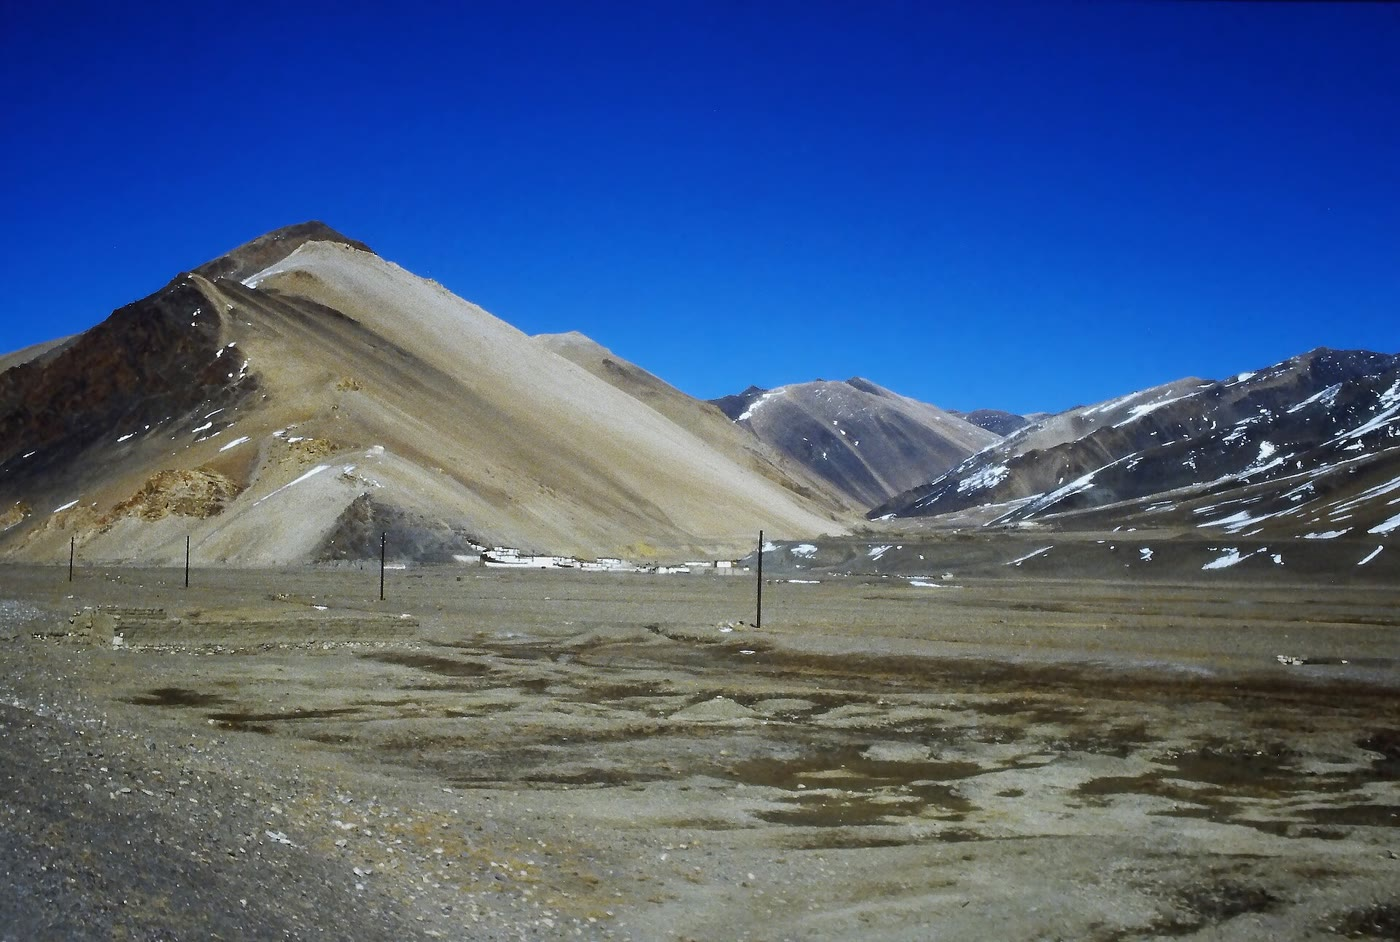
\includegraphics[width=0.66\linewidth]{images/book4/b2-14-tibet-plateau.jpg}
\par\smallskip{\small The Tibetan Plateau between Nepal and Shigatse: a flat floor of gravel and
sparse pasture, with a village, between bare mountains mantled in scree, the whole more than
four kilometres above sea level.
Photograph Jan Kranendonk, 1987, CC BY-SA 4.0.}
\end{omfigure}
% ledger: data:b4-etopo-tibet

\subsection{The weight of a plateau}

A plateau weighs on its surroundings. At every depth down to the base of its root, a column
under the plateau is under a higher pressure than a column under the lowlands next to it;
only at the compensation depth are the two equal. The high column pushes outwards.

\begin{proposition}[Excess potential energy of a plateau]\label{prop:b2:himalaya-andes:gpe}
Under the hypotheses of \cref{prop:b2:himalaya-andes:airy}, with gravity $g$, the integral of
the excess lithostatic pressure of the plateau column over the normal column, from the top
of the plateau to the compensation depth at the base of its root $r$, is
\[
  \Delta F = \rho_c g h \left(H + \frac{h}{2} + \frac{r}{2}\right) .
\]
It is the excess gravitational potential energy of the plateau column per unit area, and the
force per unit length of the plateau's edge with which the plateau pushes on its
surroundings.
\end{proposition}

\begin{proof}
Measure the depth $z$ downwards from sea level. In the plateau column the pressure is $p_1 =
\rho_c g (z + h)$ from $z = -h$ to $L = H + r$. In the normal column it is zero above sea
level, $\rho_c g z$ in the crust, and $\rho_c g H + \rho_m g (z - H)$ below. The difference $p_1
- p_0$ rises from 0 at $z = -h$ to $\rho_c g h$ at sea level; it keeps this value through the
normal crust, where both columns are crust; below $z = H$ it decreases linearly, by
$(\rho_m - \rho_c) g$ per metre, and reaches zero at $L$ since $(\rho_m - \rho_c) r = \rho_c
h$. The integral is the area of this trapezium: $\rho_c g h\,(h/2 + H + r/2)$. The work done by
the pressures when the two columns exchange matter sideways is this integral, which is why it
measures both the energy and the push.
\end{proof}

\begin{omfigure}
\centering
% figdata/bachelor-2/plateaus.py part pressure (h = 4.8 km, H = 35 km, 2700 and 3300 kg/m3)
\begin{tikzpicture}
\begin{axis}[width=0.62\linewidth, height=5.6cm, y dir=reverse, xmin=0, xmax=160, ymin=-12,
  ymax=60, xlabel={excess pressure $p_1 - p_0$ (\unit{MPa})}, ylabel={depth below sea level
  (\unit{km})}, tick label style={font=\scriptsize}, label style={font=\small},
  xtick pos=bottom, ytick pos=left, clip=false]
\addplot[fill=omThm!20, draw=omThm, line width=1pt] table[x expr=\thisrow{p_high_MPa}-\thisrow{p_ref_MPa}, y=z_km] {figdata/out/bachelor-2-plateaus-pressure.dat} \closedcycle;
\draw[dashed] (axis cs:0,0) -- (axis cs:160,0);
\draw[dashed] (axis cs:0,35) -- (axis cs:160,35);
\draw[dashed] (axis cs:0,56.6) -- (axis cs:160,56.6);
\node[font=\scriptsize, anchor=north east] at (axis cs:160,0) {sea level};
\node[font=\scriptsize, anchor=north east] at (axis cs:160,35) {normal Moho, $H$};
\node[font=\scriptsize, anchor=south east] at (axis cs:160,56.6) {base of the root, $H + r$};
\node[font=\scriptsize, anchor=west] at (axis cs:100,-8.4) {top of plateau, $-h$};
\node[font=\scriptsize, align=center] at (axis cs:60,20) {area $= \Delta F$\\$\approx\qty{6.1e12}{N.m^{-1}}$};
\end{axis}
\end{tikzpicture}
\par\smallskip{\small The excess lithostatic pressure of a plateau column over a normal
column, for $h = \qty{4.8}{km}$, $H = \qty{35}{km}$ and densities 2700 and
\qty{3300}{kg.m^{-3}}: it rises through the plateau, stays at $\rho_c g h = \qty{127}{MPa}$
through the normal crust, and falls to zero at the base of the root. The shaded area is the
excess potential energy of \cref{prop:b2:himalaya-andes:gpe}.}
\end{omfigure}
% values (plateaus.py): tibet_gpe 6.12179e12 N/m for h = 4.8

For Tibet, $r = 4.5 \times 4.8 = \qty{21.6}{km}$ and $\Delta F = 2700 \times 9.8 \times 4800
\times (35000 + 2400 + 10800) \approx \qty{6.1e12}{N.m^{-1}}$. Spread over a lithosphere
\qty{100}{km} thick, that is a mean excess stress of about \qty{60}{MPa}, of the order of the
stresses that break rocks. A plateau so heavy can no longer simply rise: it tends to spread.

\begin{definition}[Gravitational collapse]\label{def:b2:himalaya-andes:collapse}
The \emph{gravitational collapse}\index{gravitational collapse (of an orogen)} of an \omterm{def:b2:alpine-orogen:orogen}{orogen}
is the spreading of its thickened crust under its own weight, by extension of the high
regions and outward flow or thrusting at the edges, driven by the excess potential energy of
the thickened columns.
\end{definition}

Tibet is being stretched while India still pushes it. Across southern Tibet, north--south
rifts cut the plateau and accommodate east--west extension: about $9 \pm \qty{2}{mm}$ a year in
all between \ang{81} and \ang{92}~E, $1.3 \pm \qty{0.3}{mm}$ a year on the Yadong--Gulu rift
alone; north of Nepal the GPS stations show the southern plateau stretching by about
\num{12e-9} a year. Earthquakes tell the same story: thrust faulting and \omterm{def:b2:himalaya-andes:thickening}{crustal thickening}
dominate the lower ground around the plateau, strike-slip and normal faulting its interior.
Why it extends is debated. In the eastern plateau the extension has been read as \omterm{def:b2:himalaya-andes:collapse}{gravitational
collapse} driven by the weight of the plateau; in the south, others tie it to the curved shape
of the Himalayan arc, along which the thrusts diverge, or to India sliding beneath.
% ledger: wang21:rifts, ader12:extension

\subsection{Escaping sideways}

\begin{definition}[Lateral extrusion]\label{def:b2:himalaya-andes:extrusion}
\emph{Lateral extrusion}\index{lateral extrusion} (escape tectonics) is the expulsion of
blocks of crust or lithosphere sideways from a collision zone, along large strike-slip faults,
roughly perpendicular to the direction of convergence, towards a free boundary.
\end{definition}

East of Tibet, Asia is not shortened only; it is pushed aside. Long left-lateral strike-slip
faults, the Red River and the Altyn Tagh faults among them, are read as having guided the
eastward and south-eastward escape of large blocks, first the Sunda block of South-East Asia,
then Tibet and South China, while rifts and young ocean basins opened at their far ends.
Experiments in which a rigid die was pushed into a layer of plasticine produced such faults;
models that treated Asia as a continuous viscous sheet produced broad thickening instead, with
no great faults. GPS supports the motion of blocks: relative to stable Siberia, the Tarim
basin moves roughly northwards at about \qty{14}{mm} a year and South China towards the east-south-east
at about \qty{8}{mm} a year. How much of India's advance has been absorbed by thickening and how
much by extrusion is still argued.
% ledger: jiao23:extrusion

\section{The Andes}\label{sec:b2:himalaya-andes:andes}

The Nazca plate goes down beneath South America at about \qty{72}{mm} a year near
\ang{20}~S, towards the east-north-east, by the NNR-MORVEL56 angular velocities. No continent
has arrived, yet the Central Andes carry the second highest plateau on Earth.
% ledger: nnr56:poles
% values (plateaus.py): v_nazca_southamerica 72.52 mm/yr, azimuth 74.5

From west to east, between about \ang{15} and \ang{27}~S, they comprise five zones: the
\emph{forearc}; the \emph{Western Cordillera}, the volcanic arc; the high plateau, the
\emph{Altiplano} in the north and the \emph{Puna} in the south; the \emph{Eastern
Cordillera}; and the thin-skinned \omterm{def:b2:alpine-orogen:ftb}{fold--thrust belt} of the \emph{Subandean zone}, which
passes into the Chaco plain. The profile above crosses them at \ang{20}~S: from the trench,
whose deepest node lies \qty{7.7}{km} below sea level at \ang{71.4}~W, the surface climbs
more than \qty{11}{km} in about \qty{240}{km} to the edge of the plateau at \ang{69.1}~W;
the plateau stays above \qty{3000}{m} for \qty{440}{km} with a
mean of \qty{3760}{m}. The mean height is \qty{3.7}{km} in the Altiplano and \qty{4.4}{km} in
the Puna. North of \ang{23}~S the Moho is generally deeper than \qty{60}{km}; under the
central Altiplano the crust is 59 to \qty{64}{km} thick.
% ledger: gerbault05:andes, gerbault05:moho, data:b4-etopo-andes

\begin{omfigure}
\centering
\begin{tikzpicture}[x=0.56cm, y=0.38cm, font=\scriptsize]
% mantle background
\fill[gray!12] (0,-2.6) -- (5,-3.6) -- (8,-5.6) -- (10,-9.1) -- (12,-12.6) -- (13.2,-14.6) -- (26,-14.6)
  -- (26,-4.5) -- (20,-4.7) -- (17.5,-6.0) -- (15,-7.3) -- (11,-7.0) -- (9.5,-6.2) -- (8,-4) -- (5,-2)
  -- (0,-1) -- cycle;
% ocean water
\fill[blue!8] (0,0) -- (6.33,0) -- (5,-2) -- (0,-1) -- cycle;
% Nazca slab
\fill[gray!45] (0,-1) -- (5,-2) -- (8,-4) -- (10,-7.5) -- (12,-11) -- (14,-14.5) -- (13.2,-14.6)
  -- (12,-12.6) -- (10,-9.1) -- (8,-5.6) -- (5,-3.6) -- (0,-2.6) -- cycle;
% South American crust
\fill[orange!22] (5,-2) -- (8,1) -- (9,1.9) -- (10.2,2.0) -- (11,2.0) -- (15,2.0) -- (15.6,2.6) -- (16.8,2.4)
  -- (17.5,1.6) -- (20,0.6) -- (20.6,0.4) -- (26,0.3) -- (26,-4.5) -- (20,-4.7) -- (17.5,-6.0) -- (15,-7.3)
  -- (11,-7.0) -- (9.5,-6.2) -- (8,-4) -- cycle;
% Altiplano basin fill
\fill[yellow!45] (11,2.0) -- (15,2.0) -- (14.6,1.0) -- (11.4,1.0) -- cycle;
% surface line
\draw[line width=0.5pt] (0,-1) -- (5,-2) -- (8,1) -- (9,1.9) -- (10.2,2.0) -- (11,2.0) -- (15,2.0) -- (15.6,2.6)
  -- (16.8,2.4) -- (17.5,1.6) -- (20,0.6) -- (20.6,0.4) -- (26,0.3);
% arc volcanoes
\fill[red!60!black] (8.8,1.75) -- (9.2,2.9) -- (9.6,1.95) -- cycle;
\fill[red!60!black] (9.8,1.95) -- (10.2,2.8) -- (10.6,2.0) -- cycle;
\draw[red!60!black, decorate, decoration={snake, amplitude=0.6pt, segment length=4pt}] (10.8,-8.0) -- (9.9,1.6);
% Subandean decollement and splays
\draw[thick] (16.0,-1.2) -- (20.55,0.42);
\draw (17.4,-0.7) -- (17.85,1.45);
\draw (18.4,-0.35) -- (18.8,1.08);
\draw (19.4,0.0) -- (19.7,0.72);
% Moho
\draw[dashed] (8,-4) -- (9.5,-6.2) -- (11,-7.0) -- (15,-7.3) -- (17.5,-6.0) -- (20,-4.7) -- (26,-4.5);
% labels
\node at (2.6,-0.5) {Pacific};
\node at (2.4,-2.2) {Nazca plate};
\draw[-{Latex[length=1.6mm]}] (1.6,-2.8) -- (3.2,-3.0);
\node[anchor=south] (tr) at (4.3,0.9) {trench};
\draw[->] (tr.south) -- (5,-1.8);
\node[anchor=south east] at (7.6,1.0) {forearc};
\node[anchor=south, align=center] at (9.7,3.0) {Western\\Cordillera (arc)};
\node[anchor=south] at (13,2.1) {Altiplano};
\node[anchor=south, align=center] at (16.4,2.7) {Eastern\\Cordillera};
\node[anchor=south west] at (18.6,1.3) {Subandean};
\node[anchor=south] at (23.5,0.4) {Chaco plain};
\node at (13,-3.2) {thick crust};
\node at (23.2,-2.0) {Brazilian shield};
\node[anchor=north] at (23.2,-4.6) {Moho};
\node at (14.2,-9.6) {mantle wedge};
\node at (21,-10) {mantle};
\node[rotate=-50] at (12.75,-12.9) {slab};
\draw[-{Latex[length=2mm]}] (1.2,4.6) -- (0.2,4.6);
\node[anchor=south] at (0.7,4.6) {W};
\draw[-{Latex[length=2mm]}] (24.8,4.6) -- (25.8,4.6);
\node[anchor=south] at (25.3,4.6) {E};
\end{tikzpicture}
\par\smallskip{\small A schematic section across the Central Andes near \ang{20}~S (not to
scale). The Nazca plate sinks beneath the forearc; \omterm{def:b2:magma-emplacement:magma}{magma} rises from the mantle wedge (wavy
line) to the arc of the Western Cordillera; the Altiplano, with its thick basin fill, lies
between the two cordilleras, over a crust about \qty{60}{km} thick; the thin-skinned
Subandean belt is thrust eastwards over the Brazilian shield.}
\end{omfigure}
% ledger: gerbault05:andes, gerbault05:moho

\subsection{How the crust got thick}

Where did the extra crust of the Altiplano come from? The first candidate is shortening:
squeeze a strip of crust and it thickens, keeping its cross-sectional area.

\begin{proposition}[Thickening by shortening]\label{prop:b2:himalaya-andes:shortening}
Let a crust of uniform thickness $H$ be shortened, with no gain or loss of rock, into a crust
of thickness $T$ over a width $W$, the section staying parallel to the shortening. Its
original width was $W_0 = W T/H$, and the shortening is
\[
  S = W_0 - W = W\,\frac{T - H}{H} .
\]
\end{proposition}

\begin{proof}
The crust's cross-sectional area is conserved, as in the area balance of
\cref{prop:b2:alpine-orogen:balance}: $W_0 H = W T$. Hence $W_0 = WT/H$ and $S = W_0 - W =
W(T - H)/H$.
\end{proof}

At \ang{20}~S the plateau is about \qty{440}{km} wide; if its crust, about \qty{60}{km} thick,
was once \qty{35}{km}, the shortening needed is $440 \times 25/35 \approx \qty{310}{km}$.
Balanced sections near 16--\ang{21}~S find about \qty{50}{km} of shortening in the Altiplano
and more than \qty{200}{km} in the Subandean zone since the Oligocene. The crustal volumes
computed from shortening fall about \qty{20}{\percent} short of those computed from the depth
of the Moho. Part of the difference may be wrong assumptions, about the initial thickness or
the nature of the seismic Moho; part may be crust added in other ways. One compilation near
\ang{21}~S credits tectonic shortening with at least \qty{55}{\percent} of the root, the
hydration of the forearc mantle wedge with up to \qty{20}{\percent}, and magmatic addition and
tectonic erosion with only about \qty{5}{\percent}. Rock may also move inside the belt:
differences of crustal thickness create differences of potential energy, as in Tibet, and
these can drive the hot lower crust to flow from thick to thin.
% ledger: gerbault05:andes, gerbault05:volume, gerbault05:moho, data:b4-etopo-andes

\begin{omfigure}
\centering
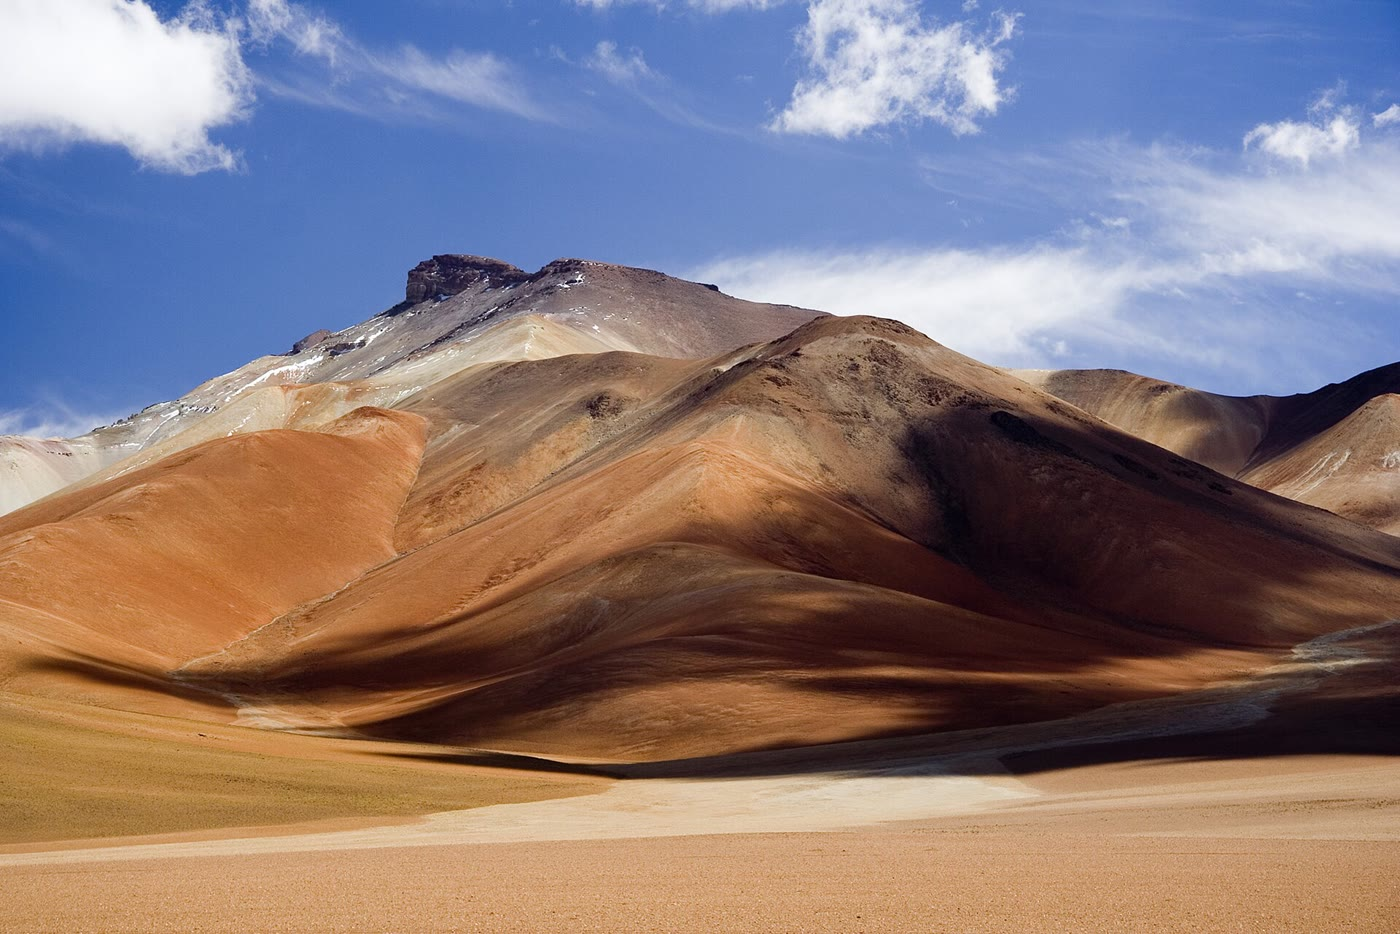
\includegraphics[width=0.66\linewidth]{images/book4/b2-14-altiplano.jpg}
\par\smallskip{\small The Bolivian Altiplano: a plain of sand and gravel at the foot of
bare hills coloured red, ochre and grey by their rocks. Photograph Luca Galuzzi, 2006, CC BY-SA 2.5.}
\end{omfigure}
% ledger: gerbault05:andes

\subsection{Flat slabs and lost roots}

The angle of the slab is not fixed, and it matters at the surface.

\begin{definition}[Flat-slab subduction]\label{def:b2:himalaya-andes:flat-slab}
\emph{Flat-slab subduction}\index{flat-slab subduction} is subduction in which the slab,
after its first descent, runs nearly horizontally beneath the overriding plate for hundreds
of kilometres before sinking again.
\end{definition}

Along the Andes, two segments of the Nazca slab are flat today, the Peruvian segment, flat
since about \qty{15}{Ma}, and the Pampean segment, since about \qty{18}{Ma}. Above them there
are no active volcanoes. When the Pampean slab flattened, the arc moved inland and erupted
less lava; above the flat segments it has fallen silent. The arc--trench gap of the Year 1 volume
explains the inland move: the gentler the slab beneath the arc, the farther from the trench it
reaches the depth at which the wedge melts; and a slab that stays flat above that depth leaves
no hot mantle wedge to melt at all.
% ledger: gauthier24:flat

\begin{definition}[Lithospheric delamination]\label{def:b2:himalaya-andes:delamination}
\emph{Lithospheric delamination}\index{lithospheric delamination} is the detachment and
sinking into the asthenosphere of the lower part of a thickened lithosphere, its mantle
lithosphere and sometimes a dense lower crust, replaced by hot asthenosphere.
\end{definition}

Delamination has been proposed beneath the southern Puna, between \ang{24} and \ang{27}~S,
about 2 to \qty{3}{Ma} ago, where young mafic lavas erupted; and along the plateau, changes
of crustal thickness and elevation have been tied to a mantle lithosphere already removed
beneath the southern Altiplano and not yet completely beneath the central Altiplano. Losing a
dense mantle lid makes the remaining column lighter: the surface rises without any more
shortening. The Puna stands about \qty{1}{km} higher than the Altiplano on a crust about
\qty{11}{km} thinner, a contrast that needs either a lighter Puna crust or a lighter mantle
beneath it.
% ledger: gerbault05:delamination, gerbault05:moho

\section{Two belts compared}\label{sec:b2:himalaya-andes:compared}

The two plateaus look alike from far away and differ in almost everything else, as the table
below gathers.

\begin{omfigure}
\centering\small
\begin{tabular}{>{\raggedright\arraybackslash}p{0.2\linewidth}|>{\raggedright\arraybackslash}p{0.34\linewidth}|>{\raggedright\arraybackslash}p{0.34\linewidth}}
 & Himalaya and Tibet & Central Andes \\ \hline
engine & continent against continent after the ocean closed & ocean plate sinking beneath a continent \\
axis & suture with \omterm{def:b2:alpine-orogen:ophiolite}{ophiolites} & volcanic arc above the slab \\
magmatism & crustal melts: \omterm{def:b2:crustal-melting:leucogranite}{leucogranites} & arc andesites; mafic lavas where the lithosphere was lost \\
convergence & about \qty{45}{mm} a year, half taken in the range & about \qty{72}{mm} a year, mostly consumed by subduction \\
great earthquakes & on the MHT, Assam 1950, $M_w \approx 8.5$ & on the subduction interface, Chile 1960, $M_w$ 9.5 \\
plateau & mean \qty{4.8}{km} over \qty{1180}{km}; crust 70--\qty{75}{km} & mean \qty{3.8}{km} over \qty{440}{km}; crust about \qty{60}{km} \\
plateau tectonics & east--west extension, extrusion & shortening on the flanks; delamination proposed \\
foreland & Indo-Gangetic foredeep and Siwalik \omterm{def:b2:alpine-orogen:foreland}{molasse} & Subandean belt and Chaco plain \\
\end{tabular}
\par\smallskip{\small The two belts side by side; the sources are cited in the sections above,
and the Chile earthquake is the largest recorded since 1900.}
\end{omfigure}
% ledger: lave00:setting, lave00:siwaliks, weinberg16:himalaya, ader12:mht, ader12:quakes, usgs:largest, gerbault05:andes, gerbault05:moho, gerbault05:delamination, nnr56:poles, data:b4-etopo-tibet, data:b4-etopo-andes, cattin01:crust, wang21:rifts, jiao23:extrusion

The deepest difference is in what goes down. In the Andes the ocean plate keeps sinking, and
most of the convergence, about \qty{72}{mm} a year, is consumed at the trench; shortening the
upper plate by \qty{310}{km} over some 30 million years would take only about \qty{10}{mm} a
year of it. In the Himalaya nothing light can sink for long, so the convergence is spent on
stacking, thickening and pushing Asia aside. Both belts grow plateaus because a thick crust
is a high crust; both plateaus stop rising when their own weight balances the push at their
edges, and then they spread.
% ledger: nnr56:poles, gerbault05:andes, ader12:mht, jiao23:extrusion

\section{How high can a mountain be?}\label{sec:b2:himalaya-andes:heights}

The highest summit, Everest, stands \qty{8848.86}{m} above sea level by the joint survey
announced in 2020. Why not twenty kilometres? A rough bound comes from the strength of rock.

\begin{proposition}[A height limit from rock strength]\label{prop:b2:himalaya-andes:height}
A column of rock of density $\rho$ standing a height $h$ above its surroundings, with no
lateral support above their level, carries at its foot a vertical stress $\rho g h$ and a
horizontal stress of zero on its free sides, hence a differential stress $\rho g h$. If the
rock fails at the differential stress $\sigma_d$, the column stands only if $h < \sigma_d/(\rho
g)$.
\end{proposition}

\begin{proof}
At the foot of the column the vertical stress is the weight of the rock above per unit area,
$\rho g h$. The sides are free, so the horizontal stress there is zero. The differential
stress is the difference of the greatest and least principal stresses, here $\rho g h - 0$.
Failure is avoided only if it stays below $\sigma_d$.
\end{proof}

A real mountain has sloping flanks that hold its core in, so the stress beneath it is
smaller; as an order of magnitude take half, $\rho g h/2$. For Everest, $2700 \times 9.8
\times 8849/2 \approx \qty{117}{MPa}$. Byerlee's law of the Year 1 volume puts the frictional
strength of rock on a fault under a normal stress of \qty{200}{MPa} at $50 + 0.6 \times 200 =
\qty{170}{MPa}$: the same order. A mountain three times higher would load its base far beyond
what rock can bear; it would fail and spread. On Earth, summits of eight to nine kilometres
are close to the limit, and a plateau, which spreads long before its summits fail, levels off
at five.
% ledger: tht:everest, byerlee:1975

\section*{Exercises}\label{sec:b2:himalaya-andes:exercises}

Data for the exercises: $g = \qty{9.8}{m.s^{-2}}$; densities of crust and mantle
\qty{2700}{kg.m^{-3}} and \qty{3300}{kg.m^{-3}} unless stated; normal crust $H =
\qty{35}{km}$.

\begin{exercise}[$\star$]\label{exo:b2:himalaya-andes:1}
A plateau stands at a mean elevation of \qty{3.0}{km}. Using
\cref{prop:b2:himalaya-andes:airy}, compute (a) its Airy root, (b) its crustal thickness.
(c) By how much would \qty{10}{km} more of crust raise it?
\end{exercise}

\begin{exercise}[$\star$]\label{exo:b2:himalaya-andes:2}
A traverse of the Himalaya of Nepal runs from the Ganges plain to the Tibetan Plateau.
(a) List, in order, the units it crosses and the faults that separate them. (b) Which fault
is a normal fault? (c) How does the metamorphic grade change northwards up to the Greater
Himalayan sequence, and then above it?
\end{exercise}

\begin{exercise}[$\star$]\label{exo:b2:himalaya-andes:3}
In central Nepal a river terrace abandoned \qty{9.2}{kyr} ago has been shortened by
\qty{196.5}{m} across the folds of the Main Frontal Thrust. (a) Compute the mean shortening
rate in millimetres a year. (b) Compare it with the GPS convergence across the range,
\qty{17.8}{mm} a year. (c) What does the agreement say about the faults north of the MFT?
\end{exercise}

\begin{exercise}[$\star$]\label{exo:b2:himalaya-andes:4}
Sort each observation into \omterm{def:b2:himalaya-andes:types}{collision orogen}, \omterm{def:b2:himalaya-andes:types}{Andean-type orogen} or both: (a) a suture lined
with \omterm{def:b2:alpine-orogen:ophiolite}{ophiolites}; (b) a line of active andesitic volcanoes; (c) \omterm{def:b2:crustal-melting:leucogranite}{leucogranites} melted from the
crust; (d) a deep oceanic trench along the front; (e) a \omterm{def:b2:alpine-orogen:foreland}{foreland basin} with \omterm{def:b2:alpine-orogen:foreland}{molasse};
(f) great earthquakes on a gently dipping fault beneath the range.
\end{exercise}

\begin{exercise}[$\star\star$]\label{exo:b2:himalaya-andes:5}
India moves at \qty{45}{mm} a year relative to Eurasia across the Himalaya; across Nepal the
range itself absorbs \qty{17.8}{mm} a year in the east and \qty{20.5}{mm} a year in the west.
(a) What fraction of the convergence does the range take in each case? (b) Where does the
rest go? (c) Over \qty{10}{Myr}, how much shortening does the remainder represent?
\end{exercise}

\begin{exercise}[$\star\star$]\label{exo:b2:himalaya-andes:6}
(a) Using \cref{prop:b2:himalaya-andes:gpe}, compute the excess potential energy of the
Altiplano, mean elevation \qty{3.7}{km}. (b) Compare it with Tibet's at \qty{4.8}{km}.
(c) Show that for a thin plateau, $h \ll H$, $\Delta F$ grows in proportion to $h$, and for a
thick one faster: what does that imply for the growth of a plateau?
\end{exercise}

\begin{exercise}[$\star\star$]\label{exo:b2:himalaya-andes:7}
(a) Compute $\rho g h/2$ beneath Everest, \qty{8848.86}{m} high, with $\rho =
\qty{2700}{kg.m^{-3}}$. (b) By Byerlee's law, $\tau = 0.85\,\sigma_n$ below \qty{200}{MPa} of
normal stress and $\tau = \qty{50}{MPa} + 0.6\,\sigma_n$ above; compute $\tau$ for $\sigma_n =
100$ and \qty{200}{MPa}. (c) What height would a strength of \qty{170}{MPa} allow, by the same
order-of-magnitude rule?
\end{exercise}

\begin{exercise}[$\star\star$]\label{exo:b2:himalaya-andes:8}
The rifts of southern Tibet take up $9 \pm \qty{2}{mm}$ a year of east--west extension between
\ang{81} and \ang{92}~E. (a) How wide is that stretch at \ang{30}~N, with \qty{111.19}{km} per
degree on a meridian? (b) Compute the mean extensional strain rate, per year and per second,
with its range. (c) Compare with the $(12.4 \pm 4.7) \times 10^{-9}$ a year found from GPS north of Nepal.
\end{exercise}

\begin{exercise}[$\star\star$]\label{exo:b2:himalaya-andes:9}
The locked Main Himalayan Thrust beneath Nepal accumulates a moment deficit of
\qty{6.6e19}{N.m} a year; the earthquakes of the last 500 years released only
\qty{0.9e19}{N.m} a year. (a) What fraction of the deficit did they release? (b) With $M_0 =
10^{1.5 M_w + 9.1}$\,\unit{N.m}, compute the moment of an $M_w$ 8.5 earthquake. (c) How often
would such earthquakes be needed to balance the deficit?
\end{exercise}

\begin{exercise}[$\star\star\star$]\label{exo:b2:himalaya-andes:10}
The Puna stands \qty{0.7}{km} higher than the Altiplano (4.4 against \qty{3.7}{km}) on a crust
\qty{11}{km} thinner. Take the Altiplano crust \qty{61.5}{km} thick and of density
\qty{2800}{kg.m^{-3}}, and a mantle of \qty{3300}{kg.m^{-3}} under both. (a) Write the
equality of the masses of the two columns above a common compensation depth. (b) Find the
density the Puna crust must have if the crust alone compensates the difference. (c) Compare
with the 150 to \qty{200}{kg.m^{-3}} quoted, and say what else could explain the contrast.
\end{exercise}

\begin{exercise}[$\star\star\star$]\label{exo:b2:himalaya-andes:11}
The volcanic front stands where the top of the slab is \qty{105}{km} deep. (a) For a slab
dipping uniformly at \ang{30}, compute the arc--trench gap with the formula of the Year 1
volume. (b) The slab now dips at \ang{30} down to \qty{90}{km}, then at only \ang{4}: compute
the new gap and the inland shift of the arc. (c) What happens to the arc if the slab flattens
at \qty{95}{km} depth and stays there for \qty{300}{km}?
\end{exercise}

\begin{exercise}[$\star\star\star$]\label{exo:b2:himalaya-andes:12}
Erosion removes about \qty{300}{km^3} of rock per kilometre of the Himalaya per million years.
India brings in crust \qty{37.5}{km} thick at \qty{21}{mm} a year. (a) How much crust per
kilometre of range per million years enters the belt? (b) What fraction does erosion remove?
(c) Where can the rest be?
\end{exercise}

\begin{problem}[{Weekend problem --- two plateaus}]\label{pb:b2:himalaya-andes:1}
The swath profiles of this chapter give the mean elevation of the nodes across Tibet
(\qtyrange{86}{90}{\degree} E) and across the Central Andes (\qtyrange{19}{21}{\degree} S).
Sampled every \ang{1.5} of latitude and every degree of longitude, rounded to \qty{10}{m}, they
read as follows. Unless stated, $g = \qty{9.8}{m.s^{-2}}$, $\rho_c = \qty{2700}{kg.m^{-3}}$,
$\rho_m = \qty{3300}{kg.m^{-3}}$ and the normal crust is $H = \qty{35}{km}$ thick.

\smallskip
\begin{center}\small
\begin{tabular}{l|ccccccccc}
latitude (\unit{\degree} N) & 26.5 & 28.0 & 29.5 & 31.0 & 32.5 & 34.0 & 35.5 & 37.0 & 38.5 \\ \hline
mean elevation (\unit{m}) & 70 & 5000 & 5030 & 4830 & 5020 & 5150 & 5050 & 4470 & 2210
\end{tabular}

\smallskip
\begin{tabular}{l|cccccccc}
longitude (\unit{\degree}) & $-71$ & $-70$ & $-69$ & $-68$ & $-67$ & $-66$ & $-65$ & $-64$ \\ \hline
mean elevation (\unit{m}) & $-3310$ & 970 & 4150 & 3720 & 3740 & 4010 & 3030 & 1170
\end{tabular}
\end{center}
\smallskip

\noindent\textbf{Part I --- Reading the profiles.}
\begin{enumerate}
\item Taking as plateau the samples above \qty{3000}{m}, compute the mean elevation of Tibet
$h_T$, rounded to \qty{0.1}{km}.
\item Do the same for the Altiplano, $h_A$, and compare with the mean height of
\qty{3.7}{km} quoted for the Altiplano and \qty{4.4}{km} for the Puna.
\item How wide is each plateau, at least, according to the samples (\qty{111.19}{km} per
degree of latitude; \qty{104.5}{km} per degree of longitude at \ang{20}~S)?
\item Compute the mean slope of the Himalayan front between \ang{26.5} and \ang{28.0}~N, as
a percentage.
\item Why is the Andean profile so much more asymmetric than the Tibetan one?
\end{enumerate}

\noindent\textbf{Part II --- Airy thicknesses.}
\begin{enumerate}[resume]
\item Compute the Airy root and the crustal thickness $T_T$ of Tibet from $h_T$.
\item Do the same for the Altiplano, $T_A$.
\item Compare with the seismic thicknesses, 70 to \qty{75}{km} under Tibet and 59 to
\qty{64}{km} under the central Altiplano. Which estimate is further off?
\item What crustal density would make Airy's thickness for Tibet equal to \qty{72.5}{km}?
\item What density would give \qty{61.5}{km} for the Altiplano?
\item Name two reasons, other than the crustal density, why a local Airy calculation can
miss the observed root.
\item The crust is \qty{37.5}{km} thick under India and \qty{72.5}{km} under Tibet. With a
density contrast at the Moho of \qty{370}{kg.m^{-3}}, estimate with the Bouguer slab, $\Delta g
= 2\pi G\,\Delta\rho\,t$, the Bouguer anomaly of Tibet's root relative to India, $t$ being the
extra thickness below sea level ($G = \qty{6.674e-11}{m^3.kg^{-1}.s^{-2}}$). Compare with the
observed difference of \qty{460}{mGal}.
\end{enumerate}

\noindent\textbf{Part III --- Shortening the Altiplano.} At \ang{20}~S the plateau is
\qty{440}{km} wide and its crust about \qty{60}{km} thick.
\begin{enumerate}[resume]
\item Using \cref{prop:b2:himalaya-andes:shortening}, compute the restored width and the
shortening needed if the crust was \qty{35}{km} thick before.
\item Balanced sections give about \qty{50}{km} of shortening in the Altiplano and
\qty{200}{km} in the Subandean zone. What fraction of the needed shortening is missing?
\item If shortening made only \qty{55}{\percent} of the extra crust, how much shortening is
needed?
\item The Subandean belt is thin-skinned. Why must its shortening still thicken the crust
somewhere?
\item Suppose the \qty{314}{km} of Part III accumulated over \qty{30}{Myr}. Compute the mean
rate, and the fraction of today's Nazca--South America convergence, \qty{72}{mm} a year, that
it represents.
\item Where does the rest of the convergence go?
\end{enumerate}

\noindent\textbf{Part IV --- The weight of Tibet.}
\begin{enumerate}[resume]
\item Using \cref{prop:b2:himalaya-andes:gpe} with $h_T$, compute Tibet's excess potential
energy per unit area.
\item Compute it for the Altiplano with $h_A$, and the ratio of the two.
\item Spread Tibet's $\Delta F$ over a lithosphere \qty{100}{km} thick: what mean stress does
it represent?
\item The extension of southern Tibet, \qty{9}{mm} a year across \qty{1060}{km}, is how much
strain a year?
\item Why can Tibet extend east--west while India still pushes it north?
\item To sum up: give the crustal thickness of Tibet computed from its mean elevation, rounded
to the kilometre, and the fraction of the seismic \qty{72.5}{km} it accounts for.
\end{enumerate}
\end{problem}
